%!TEX root = ../NCVC.tex

\mysection{基本編}
\label{sec:basic}

\subsection{CADでの作図}
\label{sec:DesignCAD}

\begin{minipage}[t]{0.4\textwidth}
 まずは基本的な加工を行うための基本的な作図方法を解説します.
図\ref{fig:sample1.jww} のような図形を書きましょう.
切削対象(ワーク)を示す矩形と,その矩形左下に円を1つ.
「NCVC」という文字は,線をつなぎ合わせたデータです.
\end{minipage}
\begin{minipage}[t]{0.6\textwidth}
\vspace*{-2zh}
\begin{figure}[H]
\centering
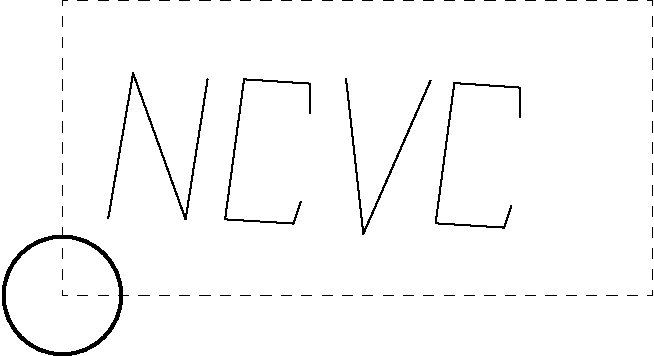
\includegraphics[scale=0.8]{No2/fig/sample1.pdf}
\caption{サンプル図形}
\label{fig:sample1.jww}
\end{figure}
\end{minipage}

\vspace*{2zh}
 NCVCはCADでの作図情報を全て読み込むのではなく,
特定のレイヤ情報を元に作図データを読み込みます.
CADでの作図において必要とされる補助線や寸法線等が加工データには必要なく,
これらを選別するための仕様です.

 その選別方法は『必要なレイヤに名前を付ける』こと.
図\ref{fig:sampleLayer.png} は図\ref{fig:sample1.jww} のレイヤ情報ですが,
0番レイヤに「ORIGIN」という名前,
1番レイヤに「CAM\_LINE」という名前を付けています.
それぞれ機械原点と切削軌跡を示し,この2つのレイヤは必須です
\footnote{実は機械原点レイヤは必須ではありません.詳細は【穴加工】の節で解説しています.}.
機械原点レイヤには工作機械のXY原点を示す円を1つだけ作図.
大きさは任意ですが,円の中心がXYの原点となります.
切削軌跡 CAM\_LINE レイヤには刃物のパス,
すなわち削りたい図形を書きます.
他,ワーク矩形を示す補助線等は別のレイヤに書きます.
レイヤに名前を付ける方法は,それぞれのCAD操作に準拠して下さい.
なお,全てのデータにおいて線種,線色は関係ありません.

\vspace*{1zh}
\begin{figure}[H]
\centering
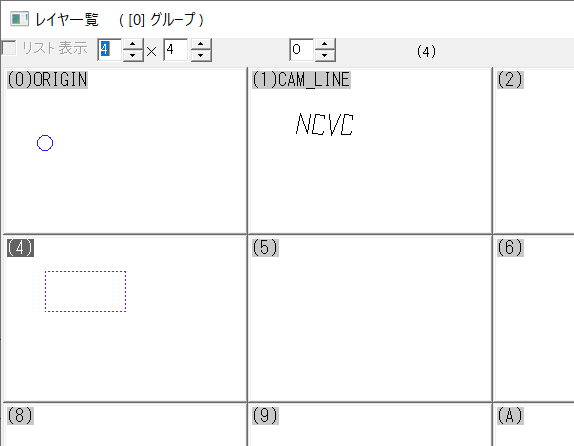
\includegraphics{No2/fig/sampleLayer.png}
\caption{レイヤ一覧}
\label{fig:sampleLayer.png}
\end{figure}

 作図が終わればCADデータをDXF形式で保存します
\footnote{
    Jw\_cadの場合,DXF形式で保存する必要はありません.NCVCはJWW形式を直接読み込むことが可能です.
    詳細は【パワーユーザ編】の【アドイン作成のすすめ】を参照して下さい.
}.
NCVCにCADデータを読み込ませるためDXF形式で保存する必要がありますが,
多くの場合,DXF形式で保存するとそのCAD独自のデータが失われるため,
使用しているCAD独自の形式でも保存しておきましょう.

\subsection{CADデータの読み込み}
\label{sec:ReadCAD}

\begin{minipage}[t]{0.5\textwidth}
 NCVCでDXF形式のCADデータを読み込みます.
が,その前に確認.
NCVCの \menu{オプション>DXF関連の設定} をクリックし,
NCVCが読み込むレイヤ名を設定して下さい.
デフォルトで先ほど設定した値になっていると思います.
基本編では[従来互換]のみ解説しますので,図\ref{fig:ReadSetup.png} の通り設定して下さい.
この値は任意です.CAD側の設定と合わせて下さい.
無事読み込めると原点を示す十字(大きさは原点円の直径)と切削対象のパスが表示されます.
原点レイヤと切削レイヤ以外に作図した情報,
例えば,図\ref{fig:sampleLayer.png} の4番レイヤに書いたワークを表す矩形は読み込まれません(図\ref{fig:ReadJWW.png}).
CADでの線種・線色は無視され,NCVCの設定に基づき表示されます.
詳細はリファレンスの表示属性を参照してください.
\end{minipage}
\begin{minipage}[t]{0.5\textwidth}
\vspace*{-2zh}
\begin{figure}[H]
\centering
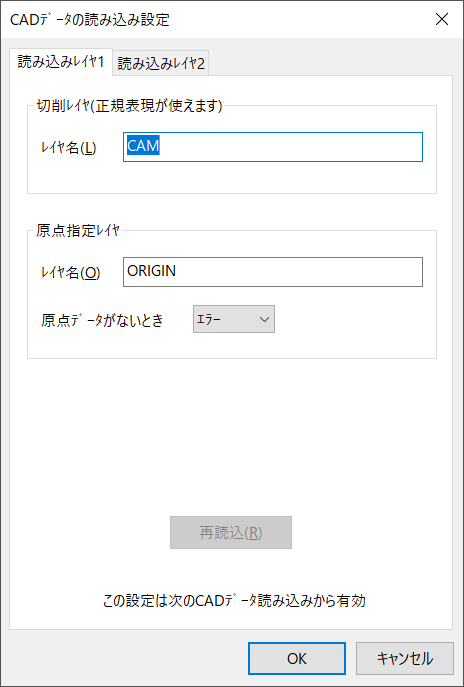
\includegraphics[scale=0.7]{No2/fig/ReadSetup.png}
\caption{読み込みレイヤ設定}
\label{fig:ReadSetup.png}
\end{figure}
\end{minipage}

\begin{figure}[H]
\centering
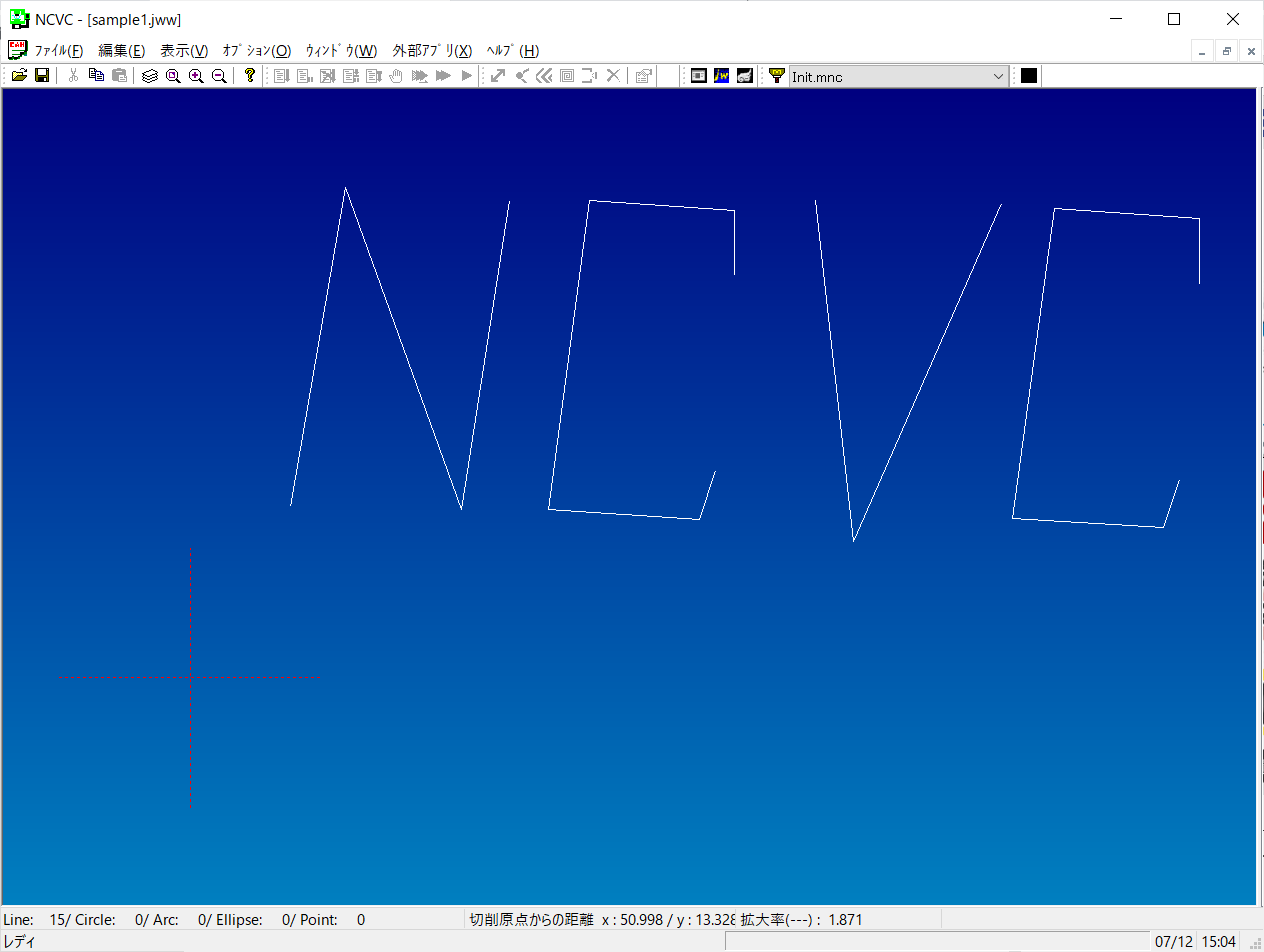
\includegraphics[scale=0.55]{No2/fig/ReadJWW.png}
\caption{CADデータの読み込み}
\label{fig:ReadJWW.png}
\end{figure}

\subsection{加工条件の設定}
\label{sec:init.nci}

 いよいよCADデータからGコードを生成するわけですが,ご覧の通り読み込んだCADデータは2次元です.
工作機械のZ軸方向の移動はどうやって制御するのでしょうか?
答えは[加工条件]の中にあります.
\menu{オプション>切削パラメータの設定} をクリックし,条件ファイル(nciファイル)を選択します.
標準で用意されている[Init.nci]の設定を変更しましょう.

 条件ファイルを選択すると図\ref{fig:init.nci.png} のダイアログが表示されます.
ここで重要なのが切削原点(G92)のZ値とR点,切り込みパラメータの3つです.

 図\ref{fig:XZ-crop.pdf} は工作機械を正面から見た図,上下にZ軸,左右にX軸です.
ワークをセットしたあと,ワーク平面を基準にZセンサー等でZ軸の位置決めを行います.
これを切削原点(G92)のZ値とします.
Zセンサーの厚みが100mmなら100と入力です.
センサーでの調整後,好みの位置に移動させてもかまいません.
無論そのときは移動した座標値を入力して下さい.

 次に切り込みですが,イメージ通り.ワークに何ミリ切り込むかという設定です.
最後にR点ですが,これは次の切削領域,この例で言うと``\,N\,''を削って``\,C\,''に移動するときのZ値を指定します.
Z軸の初期位置(原点)で移動してもかまわないのですが,初期位置は高く設定する傾向があるため,効率よく移動できる下限値と考えて下さい.
この設定ではワーク平面上空1mmの所で刃物が次の切削領域へ高速移動します.

 ワーク平面を基準に値を選びましたが,Zセンサー調整後の位置を基準,
すなわち,ワーク上空10mmの位置をZ軸の原点(G92Zをゼロ)としたとき,この例ではR点が-9mm,切り込みは-12mmとなります.
意味は同じですから各自の好みや考えやすい方で指示して下さい.

 他,主軸回転数や送り速度など,ワーク材質に合わせて設定します.

\begin{minipage}{0.5\textwidth}
\begin{figure}[H]
\centering
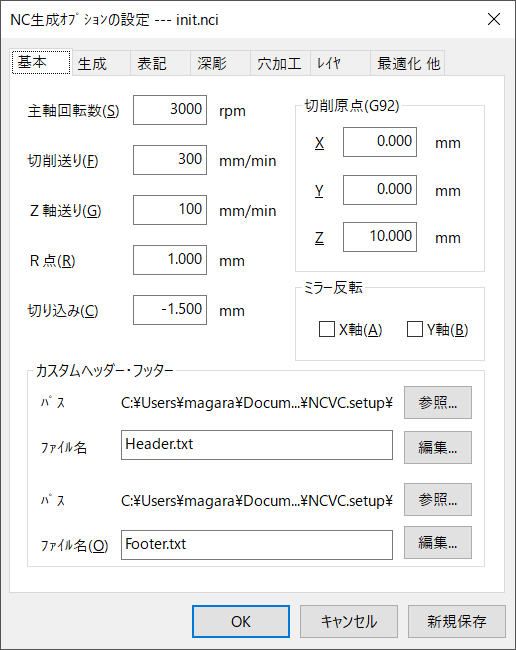
\includegraphics[scale=0.7]{No2/fig/init.nci.png}
\caption{加工条件の設定}
\label{fig:init.nci.png}
\end{figure}
\end{minipage}
\begin{minipage}{0.5\textwidth}
\begin{figure}[H]
\centering
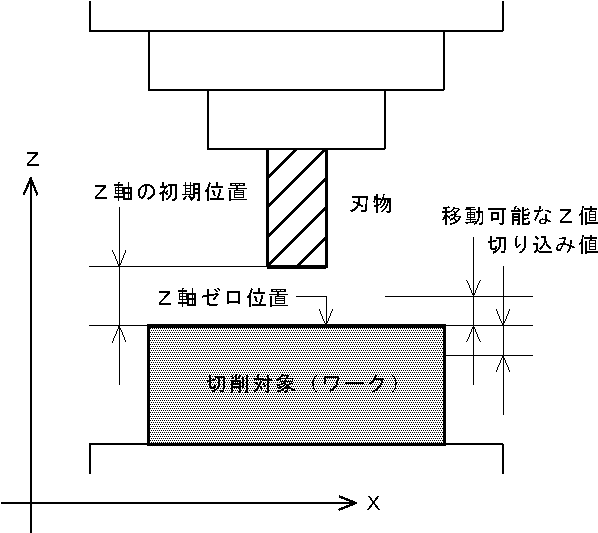
\includegraphics[scale=0.8]{No2/fig/XZ-crop.pdf}
\caption{Z軸における各パラメータの関係}
\label{fig:XZ-crop.pdf}
\end{figure}
\end{minipage}

\subsection{Gコードの生成}
\label{sec:MakeGcode}

\begin{minipage}[t]{0.5\textwidth}
 加工条件の設定ができればあとはNCVCの仕事.
\menu{ファイル>NCデータへの変換>単一条件(従来互換)} をクリック.
出力ファイル名(自動設定)と条件ファイルを指定(図\ref{fig:make.png})し,OKをクリックすれば...
\end{minipage}
\begin{minipage}[t]{0.5\textwidth}
\vspace*{-2zh}
\begin{figure}[H]
\centering
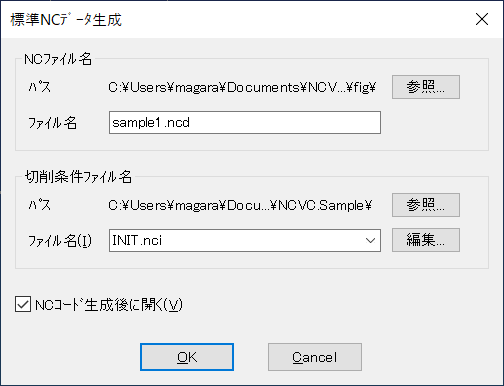
\includegraphics[scale=0.7]{No2/fig/make.png}
\caption{Gコードの出力と条件ファイルの指示}
\label{fig:make.png}
\end{figure}
\end{minipage}

\begin{figure}[H]
\centering
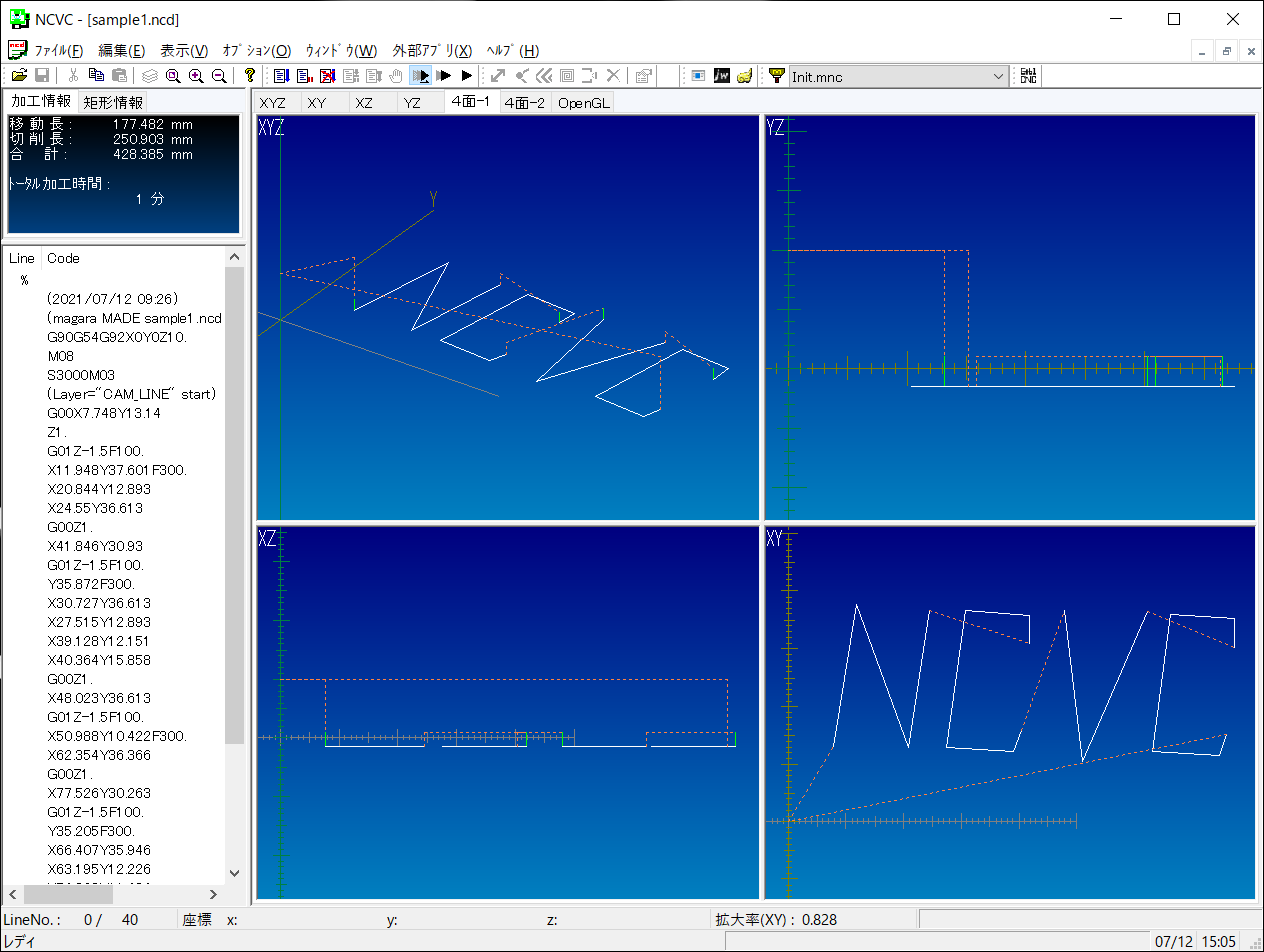
\includegraphics[scale=0.55]{No2/fig/sample01.png}
\caption{Gコードシミュレーション画面}
\label{fig:sample1.png}
\end{figure}

 おめでとうございます!見事Gコードが生成できました.
図\ref{fig:make.png} で[NC生成後に開く]にチェックが入っていると,即座に結果を確認することが出来ます.
図\ref{fig:sample1.png} にGコードのシミュレーション結果を示します.

\vspace*{3zh}
\begin{itembox}[l]{ここまでの【まとめ】}
(1) CADでの操作
\begin{itemize}
\item 工作機械のXY原点を示す円を原点レイヤに作図
\item 刃物の軌跡を切削レイヤに作図
\item 原点レイヤと切削レイヤに名前を付ける
\item 線種・線色は無視され,NCVCの表示属性により表示される
\end{itemize}
(2) NCVCでの操作
\begin{itemize}
\item CADデータを読み込むために,読み込みレイヤの設定を行う
\item Z軸の原点や切り込み量は加工条件で設定する
\end{itemize}
\end{itembox}

\newpage
\subsection{加工条件の設定2}

 ところで図\ref{fig:sample1.png} の左,Gコードのリストに注目すると,
G54ワーク座標系選択やMコードなど,CADでの作図データ以外のコードが生成されています.
これらの設定は加工条件(図\ref{fig:init.nci.png})のヘッダー・フッターの両カスタムファイルによるものです.
以下のリスト,標準で用意されているカスタムファイルで,左がヘッダー,右がフッターです.
それぞれ生成開始時と終了時に参照され,生成するGコードに併合されます.
使用できる置換キーワードなど詳細は第5章の【リファレンス】で解説します.

\begin{minipage}[t]{0.75\textwidth}
\begin{lstlisting}[caption=Header.txt,numbers=none,label=lst:header.txt]
%
({MakeDate} {MakeTime})
({MakeUser} MADE {MakeNCD} FROM {MakeDXF} AND {MakeCondition})
{G90orG91}G54{G92_Initial}
M8
{Spindle}M3
\end{lstlisting}
\end{minipage}
\begin{minipage}[t]{0.25\textwidth}
\begin{lstlisting}[caption=Footer.txt,numbers=none,label=lst:footer.txt]
M9
M5
{G0XY_Initial}
M30
%
\end{lstlisting}
\end{minipage}

\vspace*{2zh}
 テキストファイルなのでメモ帳などで編集できます.
例えばワイヤー加工機のワイヤー設定,レーザー加工機の出力設定など,ヘッダー・フッターファイルで指定しなければならない設定は多々あると思います.
実際の運用では,加工条件ファイルを含め,対象となる工作機械ごとに設定ファイルを用意する方が良いでしょう.
本解説書では標準ヘッダーにチップコンベア起動の``\,M68\,''を挿入しています.
他,そのまま使っても問題無いと思いますが,見づらいようならコメント行(ヘッダーの2~3行目)は削除してもかまいません.

 生成時に図\ref{fig:error.png} のようなエラーメッセージが出る場合があります.
特に標準のインストールパス以外にインストールされた場合,両カスタムファイルが探せませんので,加工条件にて正しいパスを設定して下さい.

\begin{figure}[H]
\centering
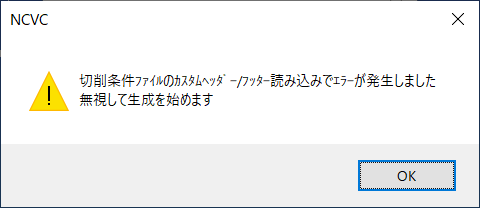
\includegraphics{No2/fig/error.png}
\caption{カスタムファイルのエラーメッセージ}
\label{fig:error.png}
\end{figure}

\subsection{Gコードの加工シミュレーション}

\subsubsection{加工時間の表示}

\begin{minipage}[t]{0.5\textwidth}
 図\ref{fig:sample1.png} の左上に注目して下さい.
[トータル加工時間]が表示されていますが,初期設定の段階では表示されません.
G01~G03(直線補間や円弧補間)等の加工時間はFパラメータとその移動距離から算出できますが,
G00早送りの移動速度は工作機械固有のパラメータです.
これをNCVCに設定することで,加工時間が算出されます.

 \menu{オプション>工作機械の設定} をクリックし機械情報ファイル(mncファイル)を選択すると図\ref{fig:kikai.png} のダイアログが表示されますので,
[位置決め(G0)移動速度]に工作機械の早送り移動速度を設定して下さい.
ここが空白の場合,加工時間は表示されません.
\end{minipage}
\begin{minipage}[t]{0.5\textwidth}
\vspace*{-2zh}
\begin{figure}[H]
\centering
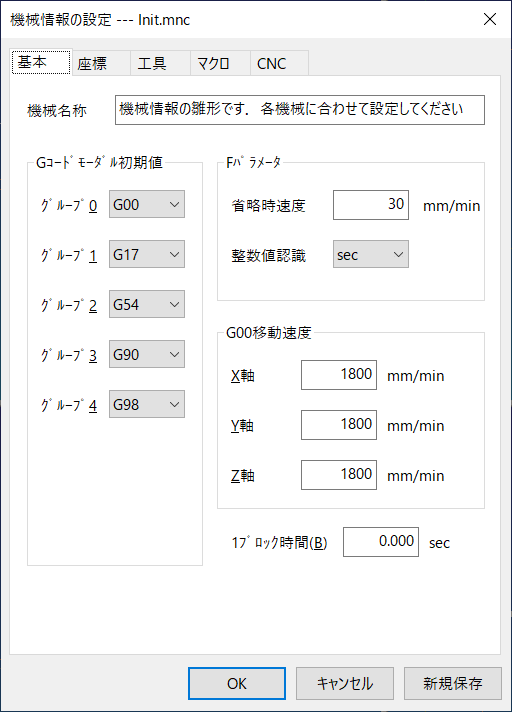
\includegraphics[scale=0.7]{No2/fig/kikai.png}
\caption{機械情報の設定}
\label{fig:kikai.png}
\end{figure}
\end{minipage}

\vspace*{2zh}
 この設定も工作機械ごとに用意しましょう.
現在選択されている機械情報ファイルはツールバーに表示されます(図\ref{fig:select.png}).
加工時間は機械情報ファイルを切り換えるたびに再計算されます.

\begin{figure}[H]
\centering
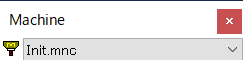
\includegraphics{No2/fig/select.png}
\caption{機械情報ツールバー}
\label{fig:select.png}
\end{figure}

\subsubsection{トレース}

 図\ref{fig:trace.png} はトレースのツールバーです.
とりあえずトレース速度を中速(右から2番目)にしてトレース実行(一番左)を押してみましょう.
どういう手順で加工されていくかを見ることができます.
トレースのスピード調整はリファレンスの表示属性を参照してください.
その他の操作については解説するまでもなく使えると思います.

\begin{figure}[H]
\centering
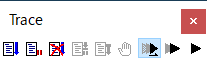
\includegraphics{No2/fig/trace.png}
\caption{トレースツールバー}
\label{fig:trace.png}
\end{figure}

\subsection{穴加工}

 基本編の最後として,固定サイクルでの穴加工データの生成を解説します.
作図レイヤは【\ref{sec:ReadCAD} CADデータの読み込み】と同じで,切削レイヤに穴加工情報を作図します.

 図\ref{fig:sample2.pdf} は矩形の四隅と中央に穴加工を行うための作図データです.
穴加工を行いたい場所を中心に,四隅には半径3mmの円,中央には半径5mmの円を作図しています.
今回はXY原点を示す原点レイヤは作図していません.

 工作機械のXY原点がワークの中央に位置し,CADデータ上でも最大占有領域の中央が原点で良い場合,NCVCがXY原点を補間する機能があります.

\begin{figure}[H]
\centering
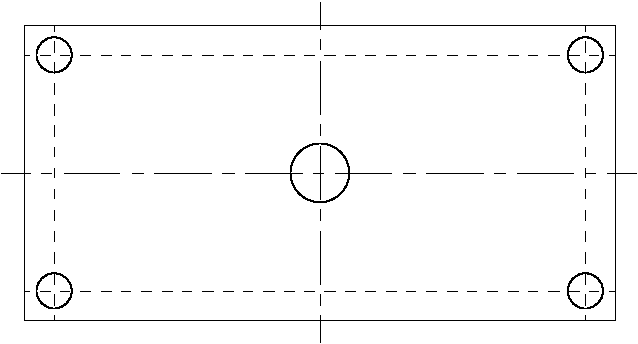
\includegraphics{No2/fig/sample2.pdf}
\caption{穴加工サンプル図形}
\label{fig:sample2.pdf}
\end{figure}

 図\ref{fig:ReadSetup.png}(p.\pageref{fig:ReadSetup.png})の読み込みレイヤ設定と違うのは,[原点データがないとき]の選択肢.
これをエラー以外に設定しておけば,NCVCがXY原点を補間します(図\ref{fig:ReadSetup2.png}).

 ただし,補間はCADデータの最大占有領域から算出されますので,意図しない位置に原点が補間される場合があります.
特別な場合を除き【\ref{sec:DesignCAD} CADでの作図】の通り原点情報を作図することを推奨します.

 穴加工に関する加工条件は【\ref{sec:init.nci} 加工条件の設定】で解説した条件ファイルの[穴加工]タブにて行います(図\ref{fig:hole.png}).
主軸回転数や切削送りなど,穴加工独自に指定可能です.
ここで注目すべき所は[拡張設定グループ]の各種項目.
[円データも穴加工データと見なす]にチェックを入れ,対象となる半径を入力することで,その中心座標に穴加工データを生成します.
従来,穴加工の入力源は点データでしたが,イメージがつかみにくい,点データをDXFに吐けないCADがある等の理由から,
円データでの穴加工が拡張設定となっています.

\vspace*{2zh}
 加工条件が設定できればあとは【\ref{sec:MakeGcode} Gコードの生成】通りです.
図\ref{fig:sample2.png} にシミュレーション結果を示します.
加工条件の[グルーピング順序]を[降順]にすることで半径の大きい中央から固定サイクル命令が生成されています.
また,[大きさごとにコメントを埋め込む]にチェックを入ることで,それぞれの半径ごとにNCVCがコメントを埋め込みますので,
手作業での修正,例えば工具交換命令を埋め込む等,編集の目安となります.

\begin{minipage}{0.5\textwidth}
\begin{figure}[H]
\centering
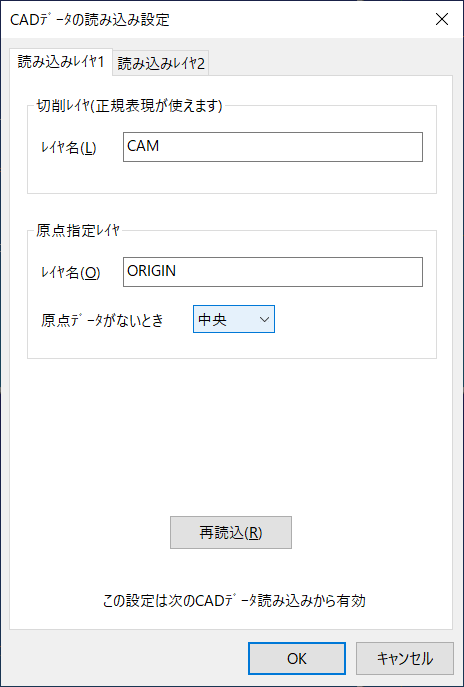
\includegraphics[scale=0.7]{No2/fig/ReadSetup2.png}
\caption{読み込みレイヤ設定2}
\label{fig:ReadSetup2.png}
\end{figure}
\end{minipage}
\begin{minipage}{0.5\textwidth}
\begin{figure}[H]
\centering
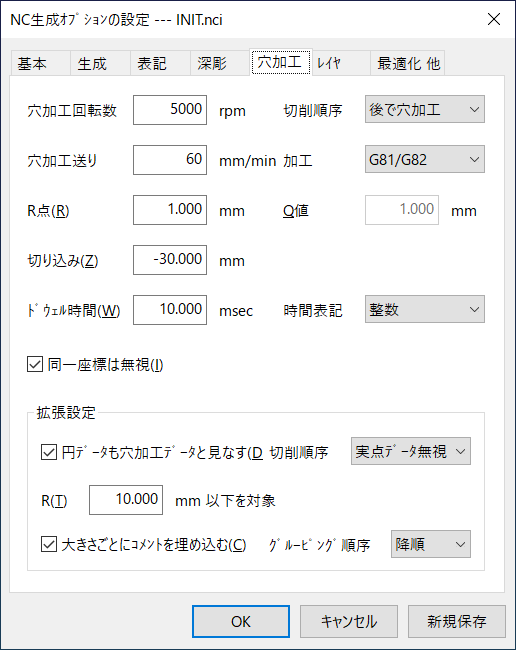
\includegraphics[scale=0.7]{No2/fig/hole.png}
\caption{穴加工の加工条件設定}
\label{fig:hole.png}
\end{figure}
\end{minipage}

\begin{figure}[H]
\centering
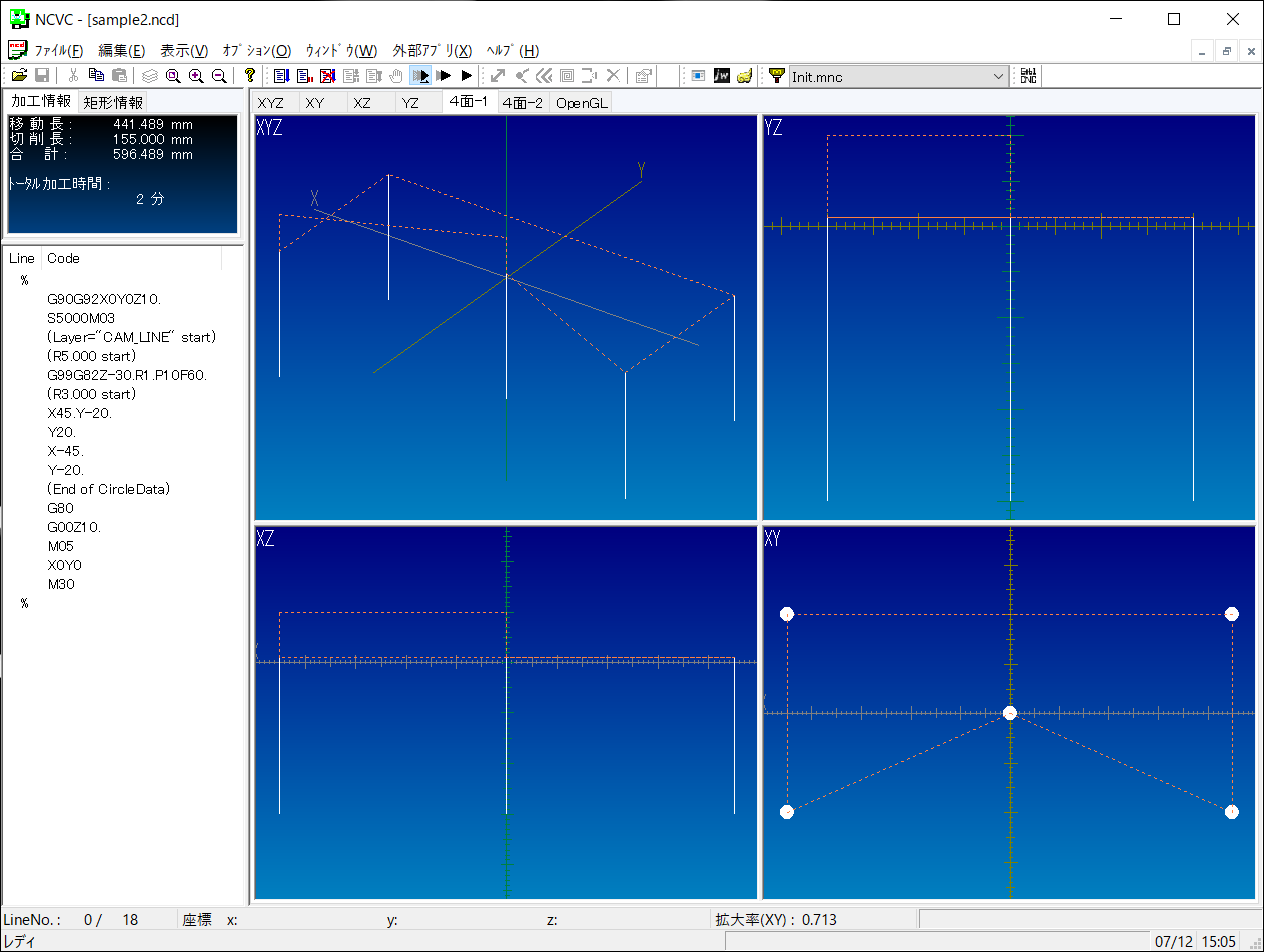
\includegraphics[scale=0.55]{No2/fig/sample02.png}
\caption{穴加工のシミュレーション画面}
\label{fig:sample2.png}
\end{figure}
